% Chapter Template

\chapter{Experiments and Evaluation}%
\label{chap:experiments_and_evaluation}

\section{Preparing Wordnets}%
\label{sec:preparing_wordnets}

In order to run our experiments we need two sets of dictionary definitions from two different languages.
Open Multilingual Wordnet~\cite{bond_linking_2013} project hosts 34 wordnets with permissive licenses on their website.\footnote{\url{http://compling.hss.ntu.edu.sg/omw/}}
We have investigated the available wordnets and found out that six of them included definitions, also known as glosses.
Since we do not use any other information related to wordnets (like semantic relationships) only definitions were extracted into a plain text corpora.
This intermediate corpora includes WordNet 3.0 synsets identifiers and the corresponding definitions in the target language.
Natural Language Toolkit~\cite{bird_natural_2009} provides an API for reading and retrieving English Princeton WordNet.
Using the synsets identifiers, it is possible to retrieve the exact synset which comes attached with an unique definition for the synset.
Finally, we have 6 aligned corpora for 6 wordnets we will run the experiments on.
Alignment here refers to definitions that represent same synset across languages appearing on the same index, a notation we will use throughout the chapter.
The statistics and the 2 letter language codes that we will commonly use to denote the wordnets for the rest of this chapter is presented in Table~\ref{tab:wordnet_stats}.

\begin{table}[hbtp]
    \centering
    \settowidth\tymin{\textbf{Language}}
    \setlength\extrarowheight{2pt}
    \begin{tabulary}{1.0\linewidth}{L L R R R R}
        \toprule
        Language Code & Language Name & Number of Definitions & Number of words & Average Words per Definition & Longest Definition \\ \midrule
        sq & Albanian & 4681 & 54980 & 11.75 & 101 \\
        bg & Bulgarian & 4959 & 63014 & 12.71 & 53 \\
        el & Greek & 18136 & 203924 & 11.24 & 89 \\
        it & Italian & 12688 & 93005 & 7.33 & 35 \\
        ro & Romanian & 58754 & 586304 & 9.98 & 105 \\
        sl & Slovene & 3144 & 39865 & 12.68 & 68 \\
        \bottomrule
    \end{tabulary}%
    \caption{Language codes and statistics for the target wordnets used in the thesis.}%
    \label{tab:wordnet_stats}
\end{table}

\section{Preparing Word Embeddings}%
\label{sec:preparing_word_embeddings}

In Chapter~\ref{chap:background_n_related}, we have mentioned the recent popularization of pre-trained word embeddings.
Initiated by word2vec\footnote{\url{https://code.google.com/archive/p/word2vec/}}, other sources for word embeddings are GloVe\footnote{\url{https://nlp.stanford.edu/projects/glove/}}, fastText\footnote{\url{https://fasttext.cc/}} and numberbatch\footnote{\url{https://github.com/commonsense/conceptnet-numberbatch}}.
Yet, word embeddings for languages other than English are scarce.
FastText hosts word embeddings for 157 languages so we used them as our primary source\cite{grave_learning_2018}.
These embeddings are trained using Common Crawl and Wikipedia data.

Numberbatch is a type of word embedding that is provided for 304 languages.
However, 10 of the available languages are presented as core languages with excellent support and 68 of them are tagged as common languages which is only given adequate support.
Referring to Table~\ref{tab:wordnet_stats}, Italian is among the core languages and the rest are in the common languages group.

The fastText embeddings include 2 million tokens out of the box.
In order to increase the efficiency of the experiments, we have cut down the size of the embeddings into 1 million and 500 thousand.
In the tables, this will be shortened into \emph{fastText 1M} and \emph{fastText 500k}.
The vectors are sorted according to their corpus frequency so the uppermost lines where the most frequent tokens of the language were used.

Numberbatch embeddings are distributed in one large file and does not include fixed number of tokens per language.
Hence after parsing the file and extracting the embeddings into individual files, the number of word vectors we are left with are presented in Table~\ref{tab:numberbatch_stats}.

\begin{table}[hbtp]
    \centering
    \begin{tabulary}{1.0\linewidth}{L R}
        \toprule
        Language Code & Number of Tokens \\
        \midrule
        bg & 20871 \\
        el & 16926 \\
        en & 417195 \\
        it & 91829 \\
        ro & 10874 \\
        sl & 11458 \\
        sq & 5512 \\
        \bottomrule
    \end{tabulary}
    \caption{The number of embeddings available in numberbatch}%
    \label{tab:numberbatch_stats}
\end{table}

These embeddings are monolingual, so they are on separate arbitrary latent spaces.
In order to represent them on the same latent space, we used VecMap~\cite{artetxe_robust_2018,artetxe_generalizing_2018,artetxe_learning_2017,artetxe_learning_2016}.\footnote{\url{https://github.com/artetxem/vecmap}}
According to \textcite{ruder_survey_2017}, bilingual or cross lingual embedding models optimize similar objectives and differences in performance is due to available data they are trained on.
\textcite{glavas_how_2019} supports this intuition and has empirically proven that common evaluation metrics like bilingual dictionary induction is not representative for the bilingual embedding's performance on downstream tasks.
Hence our preference of VecMap is highly influenced by it's availability as an open source framework and it's ease of training.

Best performing VecMap model available in the framework is supervised alignment.
It requires a bilingual dictionary, otherwise known as aligned word pairs for two languages.
We sourced our bilingual dictionary from Open Subtitles 2018\footnote{\url{http://www.opensubtitles.org/}} data as hosted by OPUS.\footnote{\url{http://opus.nlpl.eu/}}
The dictionary can be sorted by the confidence score of the translation pair, which we did so that pairs with high confidence scored swam to top.
The first 25000 translation pairs were shuffled and split into training and testing examples for 6 languages.
After supervised mapping of language specific word embedding and English word embedding, we have 6 pairs of vectors that share the same latent space, trained on 12500 word alignments.

\begin{table}[htbp]
    \centering
    \begin{tabular}{lrrr}
        \toprule
        \textbf{Language} & \textbf{FastText 1M} & \textbf{FastText 500k} & \textbf{numberbatch} \\
        \midrule
        bg & 33.61 & 35.17 & 51.97 \\
        el & 37.37 & 39.58 & 30.35 \\
        it & 58.20 & 59.28 & 50.37 \\
        ro & 37.33 & 38.71 & 64.17 \\
        sl & 21.42 & 22.91 & 74.74 \\
        sq & 24.46 & 25.36 & 58.63 \\
        \bottomrule
    \end{tabular}
    \caption{Accuracy scores (in percentage) of the word embeddings aligned using VecMap}%
    \label{tab:accuracy_results}
\end{table}

\begin{table}[htbp]
    \centering
    \begin{tabular}{lrrr}
        \toprule
        \textbf{Language} & \textbf{FastText 1M} & \textbf{FastText 500k} & \textbf{numberbatch} \\
        \midrule
        bg & 96.43 & 93.36 & 17.53 \\
        el & 94.44 & 90.28 & 12.15 \\
        it & 97.93 & 95.97 & 41.08 \\
        ro & 97.06 & 94.91 & 16.4 \\
        sl & 94.67 & 90.73 & 9.23 \\
        sq & 83.59 & 80.92 & 9.51 \\
        \bottomrule
    \end{tabular}
    \caption{Coverage scores (in percentage) of the word embeddings aligned using VecMap}%
    \label{tab:coverage_results}
\end{table}

Even though bilingual dictionary induction is not representative of a bilingual word embedding pair's performance on downstream tasks~\cite{ruder_survey_2017,glavas_how_2019}, we include the evaluation results obtained from VecMap framework as a quick measure for their quality on Table~\ref{tab:accuracy_results} for accuracy and Table~\ref{tab:coverage_results} for coverage.
Accuracy is the measure for correctly identifying the translation of a word given the test dictionary and coverage is the percentage of translation pairs that could be inducted.
From the results, it is apparent that fastText embeddings have much better coverage due to vast data they were trained on.
Yet, numberbatch exhibits better accuracy scores which might be a tradeoff of their low coverage.
Nevertheless, bilingual dictionary induction results are not indicative of word embedding's real life performance.

\section{Results}%
\label{sec:results}

In this section, we will present the results of our experiments in the order they appeared in the main text.

\subsection{Matching Results}%
\label{sub:matching_results}

In order to evaluate the definition matching of sentence embeddings that we presented in Chapter~\ref{chap:unsupervised_matching}, we choose 3 data sizes to experiment on; 2000 definitions, 3000 definitions and all available definitions each.
Table~\ref{tab:lapjv_2000} presents the 2000 definition pair experiment and Table~\ref{tab:lapjv_3000} presents the experiment with 3000 definition pairs.
As mentioned before, since definition matching is a one-to-one operation, we can only report the accuracy of the one result matched per definition.


\begin{table}[htbp]
    \centering
    \begin{tabular}{lrrr}
        \toprule
& \multicolumn{3}{c}{Percentage of Correctly Matched Definitions} \\
\cmidrule(lr){2-4}
        \textbf{Language Code} & \textbf{fastText 1M} & \textbf{fastText 500k} & \textbf{Numberbatch} \\
        \midrule
        bg & 39.35 & 40.75 & 19.00 \\
        el & 36.90 & 37.70 & 14.35 \\
        it & 27.70 & 28.25 & 36.30 \\
        ro & 38.65 & 39.45 & 20.25 \\
        sl & 14.50 & 15.05 & 5.80 \\
        sq & 54.85 & 54.15 & 27.05 \\
        \bottomrule
    \end{tabular}
    \caption{Definition matching evaluated on 2000 definition pairs}%
    \label{tab:lapjv_2000}
\end{table}

\begin{table}[htbp]
    \centering
    \begin{tabular}{lrrr}
        \toprule
& \multicolumn{3}{c}{Percentage of Correctly Matched Definitions} \\
\cmidrule(lr){2-4}
        \textbf{Language Code} & \textbf{fastText 1M} & \textbf{fastText 500k} & \textbf{Numberbatch} \\
        \midrule
        bg & 35.27 & 36.00 & 18.10 \\
        el & 36.13 & 36.07 & 11.70 \\
        it & 24.67 & 24.90 & 32.07 \\
        ro & 36.43 & 36.87 & 18.73 \\
        sl & 11.27 & 11.40 & 4.63 \\
        sq & 39.43 & 39.67 & 19.03 \\
        \bottomrule
    \end{tabular}
    \caption{Definition matching evaluated on 3000 definition pairs}%
    \label{tab:lapjv_3000}
\end{table}

\begin{table}[htbp]
    \centering
    \begin{tabular}{@{}lrrr@{}}
        \toprule
 & \multicolumn{3}{l}{Percentage of Correctly Matched Definitions} \\ \cmidrule(l){2-4}
 & \textbf{fastText 1M} & \textbf{fastText 500k} & \textbf{Numberbatch} \\ \midrule
        \textbf{Best} & 54.85 & 54.15 & 36.30 \\
        \textbf{Worst} & 11.27 & 11.40 & 4.63 \\
        \textbf{Average} & 32.93 & 33.35 & 18.92 \\
        \bottomrule
    \end{tabular}
    \caption{The summary of matching dictionary definitions}%
    \label{tab:lapjv_summary}
\end{table}

In order to assess the feasibility of this algorithm in a real life data, we ran the experiment using all of the available dictionary definitions.
We present the results in Table~\ref{tab:lapjv_full}.

Romanian wordnet definitions did not fit into the memory of the machine we tested on (64 GB of available RAM) so we could not present the full definition matching results for Romanian wordnet.

\begin{table}[htbp]
    \centering
    \begin{tabulary}{0.8\linewidth}{L r R}
        \toprule
        \textbf{Language Code} & \textbf{Definitions} & \textbf{Percentage of Definitions Matched Correctly} \\ \midrule
        bg & 4958 & 28.52 \\
        el & 18105 & 31.06 \\
        it & 12585 & 15.65 \\
        sl & 3143 & 11.42 \\
        sq & 4680 & 44.81 \\
        \bottomrule
    \end{tabulary}
    \caption{Definition matching using all the available definition in the corpora}%
    \label{tab:lapjv_full}
\end{table}

\subsection{Monolingual Retrieval Results}%
\label{sub:chap4_results}

We have presented our method of translating the target wordnet definitions into English and running monolingual document retrieval on the corpora in Section~\ref{sec:monolingual_retrieval}.
As mentioned before, we handled the original English definitions as the document collection to retrieve from and used the translated target wordnet definitions as queries.
We truncated the definitions to 2000 pairs each and ran the experiment.

The results are presented in Table~\ref{tab:monolingual_tfidf}.
Considering the other approaches, \tfidf{} weighted term document matrices and cosine similarity between definitions does not seem adequate for solving the task at hand.
Mean reciprocal rank penalizes the query according to the rank of the correct result, if the correct definition is retrieved on a lower rank, the MRR diminishes.
The divide between the MRR score and the precision at 1 score indicates that for some definitions the noise that arises from the translation keeps the correct definition from appearing among the top results heavily.

\begin{table}[htbp]
    \centering
    \begin{tabulary}{1.0\linewidth}{L R R R R R}
        \toprule%
        \textbf{Language Code} & \textbf{MRR} & \textbf{Precision at 10} & \textbf{Precision at 10 \%} & \textbf{Precision at 1} & \textbf{Precision at 1 \%} \\
        \midrule%
        bg & 0.087 & 674 & 0.337 & 403 & 0.202 \\
        el & 0.122 & 1006 & 0.503 & 709 & 0.355 \\
        it & 0.016 & 476 & 0.238 & 250 & 0.125 \\
        ro & 0.051 & 988 & 0.494 & 728 & 0.364 \\
        sl & 0.073 & 584 & 0.292 & 317 & 0.159 \\
        sq & 0.056 & 979 & 0.490 & 767 & 0.384 \\
        \bottomrule
    \end{tabulary}
    \caption{Experiment results for monolingual retrieval, ran on 2000 definition pairs}%
    \label{tab:monolingual_tfidf}
\end{table}

\subsection{Cross Lingual Document Retrieval Results}%
\label{sub:cross_lingual_retrieval_results}

We present the results of the method we have presented in Section~\ref{sec:cross_lingual_document_retrival} on the Table~\ref{tab:cldr_results}.
We handle out of vocabulary words in the experiment data simply by omitting them.
The vocabulary column shows the number of tokens available for the corresponding language given the type of vector used.
Also, we did not include definitions with less than 2 tokens in the experiments in order to avoid using potentially unrepresentative definitions as well as keeping the problem on the short document retrieval instead of dictionary induction domain.
MRR scores are given as percentages.
Due to space restrictions, we omitted the language code header and used \enquote{\%} as the percentage of precision at one metric identifier.

\begin{landscape}
    \begin{table}[htbp]
        \centering
        \begin{tabular}{llr|rr|rr|rr|rr}
            \toprule
 &  &  & \multicolumn{2}{r}{\textbf{WMD tf-idf}} & \multicolumn{2}{r}{\textbf{Sinkhorn tf-idf}} & \multicolumn{2}{c}{\textbf{WMD tf}} & \multicolumn{2}{c}{\textbf{Sinkhorn tf}} \\ \cline{4-11}
 & \textbf{Vector} & \textbf{Vocabulary} & \multicolumn{1}{c}{\textbf{MRR}} & \multicolumn{1}{c}{\textbf{\%}} & \multicolumn{1}{c}{\textbf{MRR}} & \multicolumn{1}{c}{\textbf{\%}} & \multicolumn{1}{c}{\textbf{MRR}} & \multicolumn{1}{c}{\textbf{\%}} & \multicolumn{1}{c}{\textbf{MRR}} & \multicolumn{1}{c}{\textbf{\%}} \\ \cline{2-11}
            \multirow{3}{*}{bg} & 1M FastText & 10532 & 50.83 & 41.50 & 51.85 & 42.65 & 41.81 & 33.95 & 42.76 & 34.60 \\
                                & 500k FastText & 10457 & 51.15 & 41.90 & 52.24 & 43.00 & 42.18 & 34.15 & 43.19 & 34.80 \\
                                & Numberbatch & 6028 & 25.32 & 17.45 & 24.97 & 17.15 & 18.55 & 12.30 & 18.09 & 11.35 \\ \cmidrule(lr){2-11}
            \multirow{3}{*}{el} & 1M FastText & 9307 & 47.82 & 39.05 & 48.67 & 40.15 & 40.74 & 32.85 & 41.42 & 33.40 \\
                                & 500k FastText & 9168 & 47.45 & 38.45 & 48.45 & 39.95 & 40.53 & 32.55 & 41.39 & 33.55 \\
                                & Numberbatch & 5127 & 19.92 & 13.15 & 20.06 & 13.40 & 14.71 & 9.95 & 14.94 & 10.00 \\ \cmidrule(lr){2-11}
            \multirow{3}{*}{it} & 1M FastText & 10025 & 40.24 & 31.15 & 40.60 & 31.45 & 31.98 & 23.50 & 32.07 & 23.40 \\
                                & 500k FastText & 9975 & 40.27 & 31.15 & 40.49 & 31.30 & 32.11 & 23.65 & 32.21 & 23.50 \\
                                & Numberbatch & 8875 & 42.72 & 33.30 & 42.77 & 33.35 & 35.11 & 26.70 & 35.12 & 26.80 \\ \cmidrule(lr){2-11}
            \multirow{3}{*}{ro} & 1M FastText & 12165 & 51.30 & 41.60 & 51.95 & 41.50 & 44.20 & 35.90 & 45.06 & 35.60 \\
                                & 500k FastText & 12034 & 51.28 & 41.65 & 52.37 & 42.20 & 43.85 & 35.50 & 45.14 & 35.75 \\
                                & Numberbatch & 6939 & 27.68 & 19.85 & 27.70 & 19.80 & 21.57 & 15.70 & 21.86 & 16.25 \\ \cmidrule(lr){2-11}
            \multirow{3}{*}{sl} & 1M FastText & 12185 & 26.22 & 17.80 & 26.38 & 18.05 & 23.43 & 15.10 & 23.97 & 15.60 \\
                                & 500k FastText & 12020 & 26.12 & 17.80 & 26.31 & 17.95 & 23.47 & 15.15 & 24.03 & 15.80 \\
                                & Numberbatch & 5870 & 9.35 & 4.80 & 9.46 & 5.00 & 6.35 & 2.90 & 6.26 & 2.85 \\ \cmidrule(lr){2-11}
            \multirow{3}{*}{sq} & 1M FastText & 8048 & 65.66 & 59.15 & 63.97 & 56.40 & 56.47 & 48.55 & 56.94 & 49.30 \\
                                & 500k FastText & 7990 & 65.61 & 58.70 & 64.42 & 56.85 & 56.61 & 48.80 & 57.05 & 49.25 \\
                                & Numberbatch & 4908 & 31.07 & 23.55 & 31.06 & 23.30 & 24.31 & 17.80 & 24.74 & 18.35 \\
                                \bottomrule
        \end{tabular}
        \caption{Results of cross lingual document retrieval cast as dictionary alignment}%
        \label{tab:cldr_results}
    \end{table}
\end{landscape}

\subsection{Performance Comparison}%
\label{sub:performance_comparison}

\textcite{balikas_cross-lingual_2018} suggested entropic regularized version of word mover's distance.
Their claim was that the smoothed out matrix can be solved more efficiently using the Sinkhorn-Knopp algorithm~\cite{sinkhorn_concerning_1967}.
Since the original study did not report on timing performance results, we have timed our experiments and aligned our 6 corpora using different number of definition pairs.
After obtaining the embeddings, only timing information was relevant so we averaged the results over the experiments that used the same number of instances.
We cannot repeat the experiment using increasing number of definition pairs since the number of definitions available within each language's wordnet is restrictive.
So we ran the timing study for 100, 200, 500 and 1000 definition pairs.
To our surprise, there were next to no differences in terms of MRR or precision at one between Sinkhorn and word mover's distance when the other variables were fixed.
Yet, using Sinkhorn algorithm as suggested by \citeauthor{balikas_cross-lingual_2018} results in an average slowdown of 2.52 regarding our experiments.
We present Figure~\ref{fig:perf} to compare the timings of two equally performing approaches.

\begin{figure}[htpb]
    \centering
    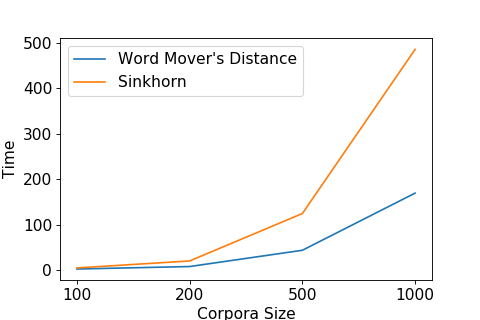
\includegraphics[width=1\linewidth]{perf.png}
    \caption{Timing comparison between word mover's distance and Sinkhorn algorithm}%
    \label{fig:perf}
\end{figure}

%%%%%%%%%%%%
%  IN DOMAIN EMBEDDINGS  %
%%%%%%%%%%%%%%%%%%%%%%%%%%
\section{Investigating Word Embedding Sources}%
\label{sec:investigating_word_embedding_sources}

We experimented with in domain \emph{fastText} embeddings in order to ask if pre-trained embeddings are better than embeddings trained on the experiment data.
Since Romanian wordnet has the most data available, we have trained Romanian embeddings on the Romanian wordnet definitions, mapped the embeddings to the same latent space using supervised VecMap and ran cross lingual document retrieval experiments using word mover's distance and Sinkhorn.
Compared to MRR score of 51.30 for the word mover's distance and 51.95 with the Sinkhorn algorithm, using word embeddings trained using available data resulted in an MRR score of 28.69 for word mover's distance and 28.6 for Sinkhorn.
Considering the drop in performance, we did not repeat the experiments for other language's corpora.

\section{Supervised Encoding Results}%
\label{sec:supervised_encoding_results}

In order to train our supervised dictionary definition encoder, we used Keras~\cite{chollet_keras_2015}.
All the available definitions were used for this task so refer to Table~\ref{tab:wordnet_stats} for the details.
Romanian wordnet includes the highest number of definitions, followed by Greek and Italian.
Since the task is supervised, we would expect the highest accuracy from those wordnets.

We trained our models over 200 epochs but the accuracy and training loss plateau after 50 epochs so we only report up to \nth{50} epoch on our figures to reflect that.
Due to highest coverage of tokens, we ran the supervised experiments using fastText embeddings, truncated to 1 million tokens.
Learning rate of the model initialized on 1 and adapted dynamically.
The plateau were hit as the learning rate adapted to 0.01.
The input for the network was chosen as 25 words.
Definitions that were longer than 25 words were truncated.
The dimensions of the LSTM layer was selected as 100 which encoded fastText embeddings on 300 dimensions.

We present the training and \emph{validation} accuracy results on Figure~\ref{fig:LSTM_Acc}
The training and validation \emph{loss} are presented in Table~\ref{fig:LSTM_loss}

\begin{figure}[htpb]
    \centering
    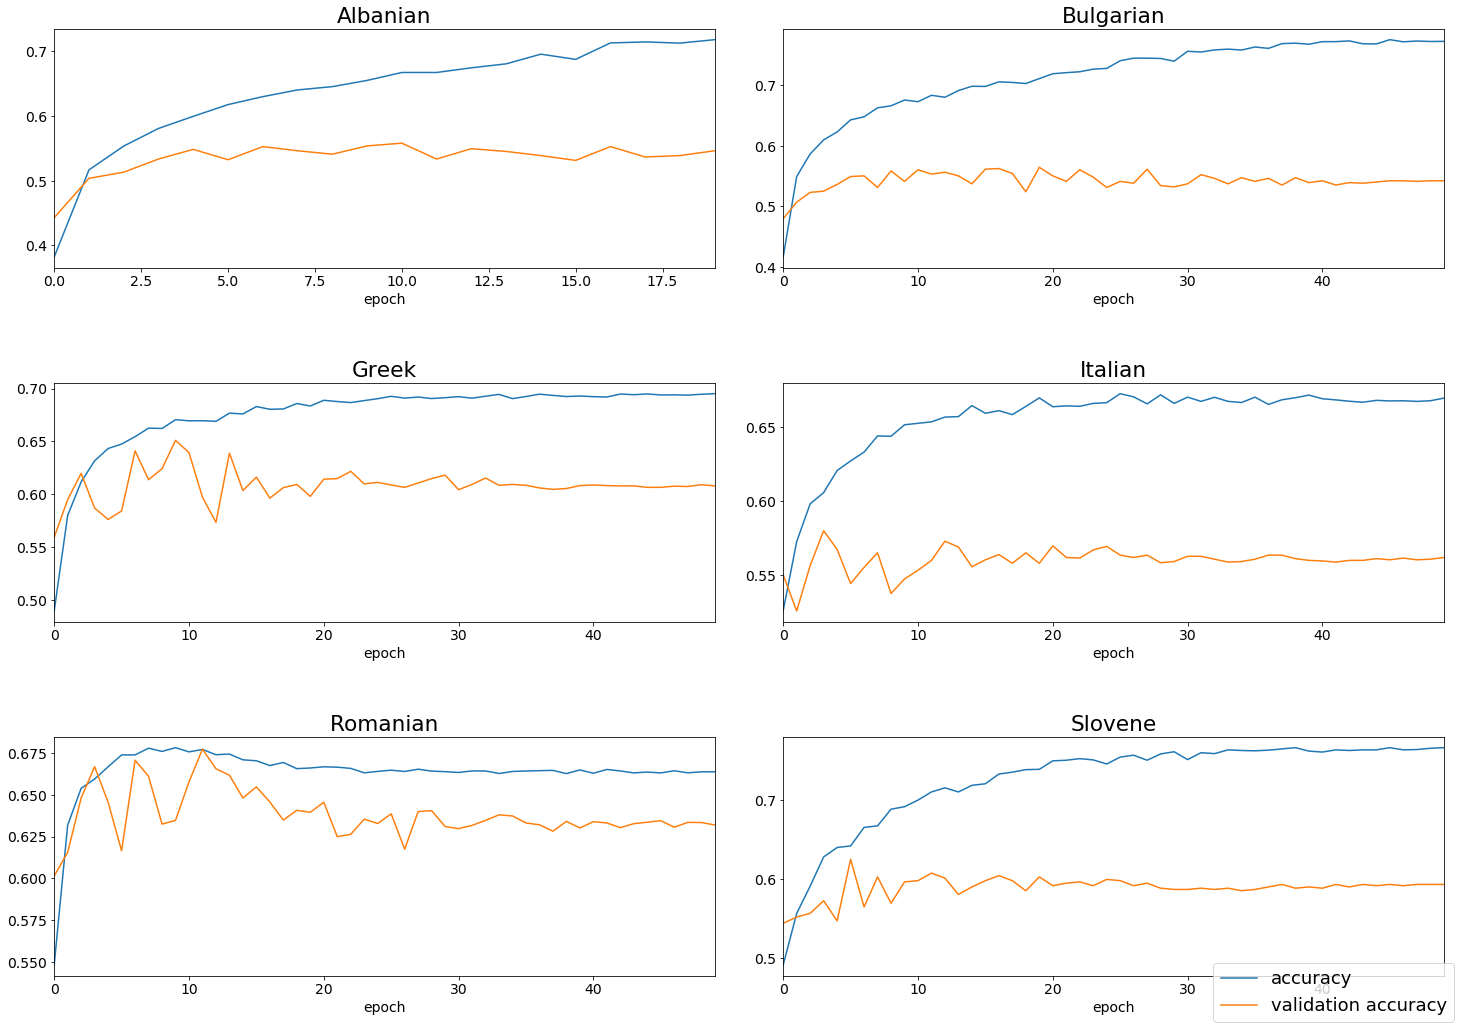
\includegraphics[width=1\linewidth]{LSTM_Acc.png}
    \caption{Accuracy of the supervised encoder on 6 wordnet corpora}%
    \label{fig:LSTM_Acc}
\end{figure}


\begin{figure}[htpb]
    \centering
    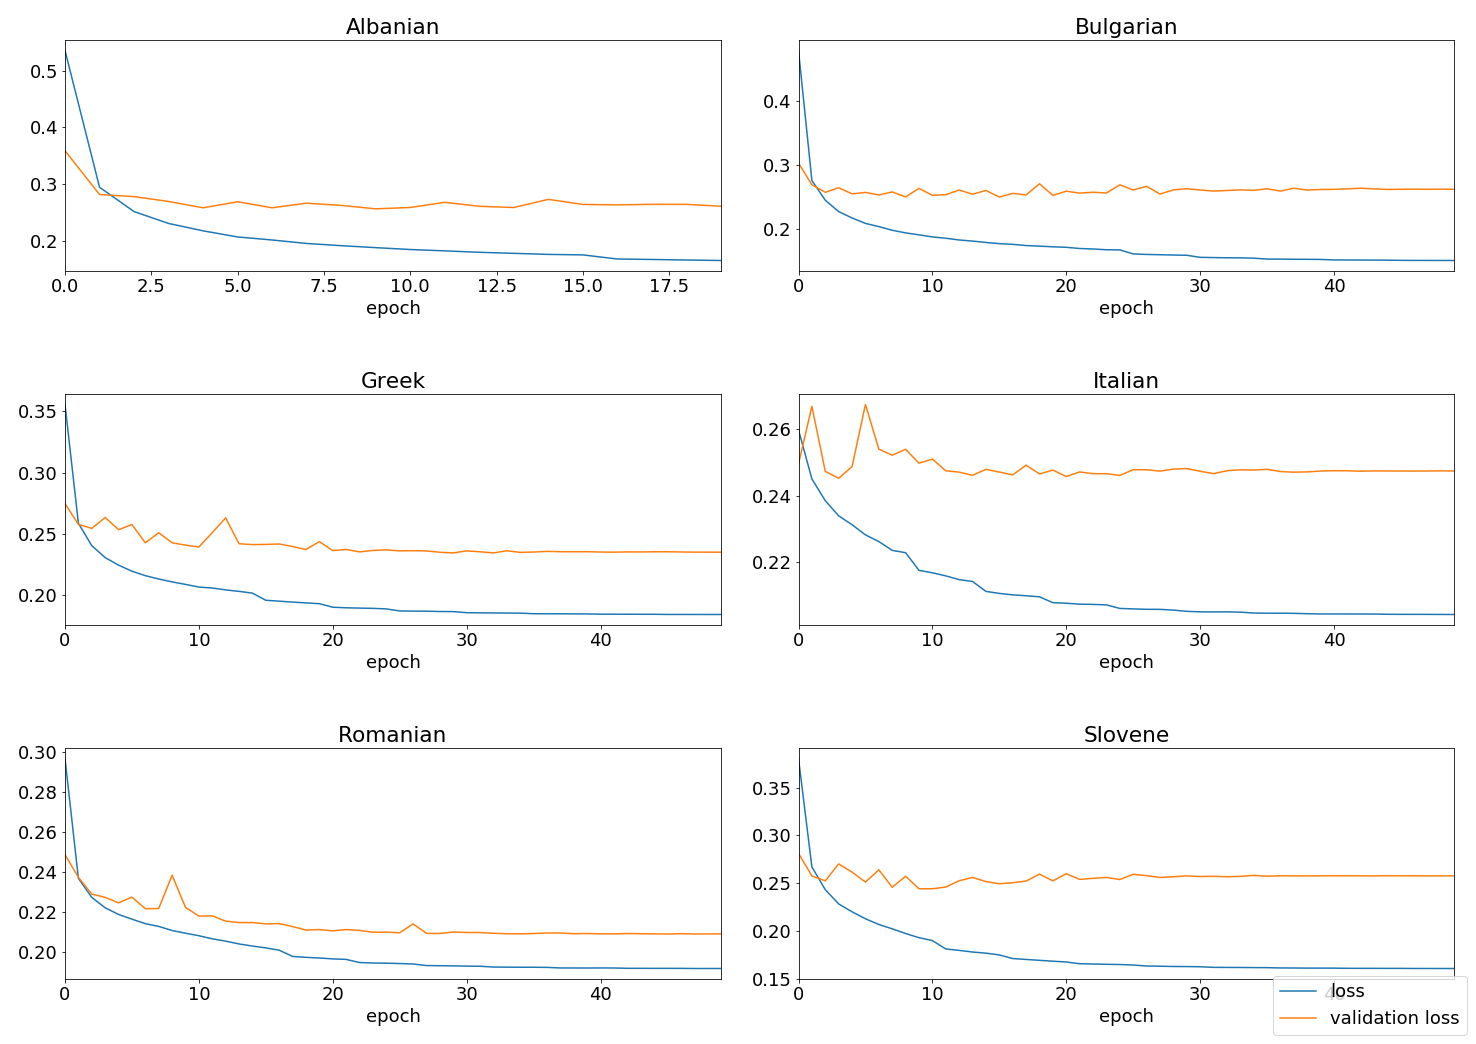
\includegraphics[width=1\linewidth]{LSTM_Loss.png}
    \caption{Loss of the supervised encoder on 6 wordnet corpora}%
    \label{fig:LSTM_loss}
\end{figure}

Overall, we achieved the best validation accuracy, the accuracy on definitions that were never seen in training data with the language that has the highest number of training data avaiable, Romanian.
After 15 epochs of training, accuracy of 65\% is achieved and the accuracy fluctuates around 63\% after \nth{30} epoch.
Surprisingly, the encoder's performance was comparable among Bulgarian and Italian even though the latter has less than half the data available to train than Italian.

\begin{table}[htbp]
    \centering
    \begin{tabulary}{1\linewidth}{L R R}
        \toprule
        Language Code & Dictionary Size & Accuracy After Plateau  \\
        \midrule
        bg & 4959 & 0.56  \\
        el & 18136 & 0.60  \\
        it & 12688 & 0.56  \\
        ro & 58754 & 0.64  \\
        sl & 3144 & 0.59  \\
        sq & 4681 & 0.53 \\
        \bottomrule
    \end{tabulary}
    \caption{The relation between the validation accuracy and the number of data points}%
    \label{tab:lstm_size_acc}
\end{table}

%%%%%%%%%%%%%%%%
%  CASE STUDY  %
%%%%%%%%%%%%%%%%
\section{Case Study}%
\label{sec:case_study}

In order to test our approach, we acquired a general purpose Turkish dictionary, to be used solely for research purposes.
The dictionary was in a proprietary format so we have parsed the terms alongside their definitions.
The parts of speech for the terms are also extracted.
All in all, 67351 headwords with 93062 definitions are obtained.

We have shown that the approaches we have presented so far are bound by their memory restrictions.
We have tried to overcome it by running the experiment on only nouns but the issue persisted for the case study as well.
As a result, we referred to \textcite{khodak_automated_2017} and constrained our scope to a list of core WordNet synsets.
Open Multilingual Wordnet hosts~\footnote{\url{http://compling.hss.ntu.edu.sg/omw/wn30-core-synsets.tab}} a list that identifies 4961 WordNet identifiers in the form of offset and part of speech that is compatible with the nltk library.
The list has been prepared in \textcite{boyd-graber_adding_2006} by human evaluators by selecting salient synsets from a list of frequent words.
By using a core WordNet, we picked ourselves a problem domain we can tackle.
We also deleted the identifiers for verbs and adjectives and worked only with nouns.
Then, the experiment set for the Turkish dictionary is selected by translating the lemmas that belong to core WordNet synsets to Turkish and using the resulting set to query the headwords of the Turkish dictionary.
Using this method, we obtained 702 Turkish definitions and 3280 WordNet definitions.

The methods we studied so far work with two corpora of the same size so we randomly picked 702 English WordNet definitions to go against 702 Turkish dictionary definitions.
We use our best performing set of approaches; word mover's distance using \tfidf{} weights, run on fastText embeddings mapped using VecMap.
The bilingual dictionary provided by OpenSubtitles used in order to map Turkish and English fastText embeddings.

While preparing the corpora for the word mover's distance, 101 Turkish definitions are dropped due to them having no words to be represented by fastText embeddings.
Same number of English WordNet definitions are also dropped to keep to the symmetric size constraint.
Then, word mover's distance is run over 601 Turkish and English definitions.

We do not know the ground truth for the mapping in this study hence we cannot report for any evaluation metric.
As a result, in Appendix~\ref{app:case_study}, we present 100 randomly selected pairs, English definitions that were retrieved as the top result against the respective Turkish query.
